%\documentclass[sn-mathphys,Numbered]{sn-jnl}% Math and Physical Sciences Reference Style
\documentclass[pdflatex,sn-mathphys-num,Numbered]{sn-jnl}% Math and Physical Sciences Numbered Reference Style 

\usepackage{graphicx}%
\usepackage{multirow}%
\usepackage{amsmath,amssymb,amsfonts}%
\usepackage{amsthm}%
\usepackage{mathrsfs}%
\usepackage[title]{appendix}%
\usepackage{xcolor}%
\usepackage{textcomp}%
\usepackage{manyfoot}%
\usepackage{booktabs}%
\usepackage{algorithm}%
\usepackage{algorithmicx}%
\usepackage{algpseudocode}%
\usepackage{listings}%
\theoremstyle{thmstyleone}%
\newtheorem{theorem}{Theorem}%  meant for 
\newtheorem{proposition}[theorem]{Proposition}% 
\theoremstyle{thmstyletwo}%
\newtheorem{example}{Example}%
\newtheorem{remark}{Remark}%
\theoremstyle{thmstylethree}%
\newtheorem{definition}{Definition}%
\usepackage[T1]{fontenc}

\raggedbottom

\begin{document}

\title[Article Title]{Matrix-based imaging through dynamic scattering - Supplementary Materials}

\author[1]{\fnm{Elad} \sur{Sunray}}
\equalcont{These authors contributed equally to this work.}

\author[1]{\fnm{Gil} \sur{Weinberg}}
\equalcont{These authors contributed equally to this work.}

\author[1]{\fnm{Benzy} \sur{Laufer}}
\equalcont{These authors contributed equally to this work.}

\author*[1]{\fnm{Ori} \sur{Katz}}\email{orik@mail.huji.ac.il}


\affil[1]{\orgdiv{Institute of Applied Physics}, \orgname{The Hebrew University of Jerusalem}, \orgaddress{\city{Jerusalem}, \postcode{9190401}, \country{Israel}}}

\maketitle

% \noindent\textbf{This PDF file includes:}

% Materials and Methods

% Supplementary Text

% Figs. S1 to S3

% Full Reference List\\


% \newpage
% \tableofcontents

\newpage


\section{Point spread functions estimation by frame-wise deconvolution}

Since in isoplanatic imaging, each captured frame $I_m$ is given by a convolution of the object, $O$, with the relevant PSF, $P_m$: $I_m = P_m * O$. Once I-CLASS retrieves the object, the PSF can be estimated by deconvolving each frame with the recovered object. 
This approach enables a study of the temporal dynamics of the medium from the estimated PSFs throughout the multi-frame video acquisition. To demonstrate this, we present two examples from the incoherent imaging experiments using Wiener deconvolution in Fig.~\ref{fig_S1} and supplementary videos S1 and S2, corresponding to the frames shown in Fig.~2b-e and 2f-i, respectively, in the main text. Fig.~\ref{fig_S1}a,d shows a few raw captured frames, Fig.~\ref{fig_S1}b,e show the reconstructed objects, and Fig.~\ref{fig_S1}c,f show the estimated PSFs for each camera frame obtained using a Wiener deconvolution.


%%%%%%%%%%%%%%% Figure s1 - PSFs estimation using deconvolution %%%%%%%%%%%%%%%%%%%%%%
\begin{figure}[htb!]
	\centering
	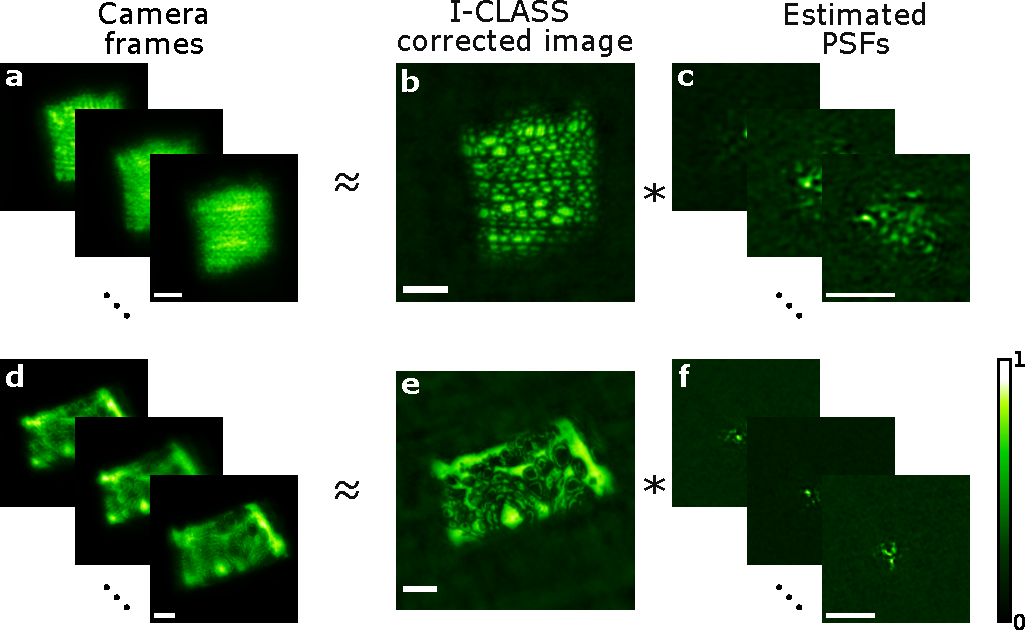
\includegraphics [width=0.98\textwidth,]
	{supp_figures/figure_S1.pdf}
         \renewcommand{\thefigure}{S1}

    \caption{\textbf{Frame-wise estimation of time-varying PSFs using Wiener deconvolution}. \textbf{a,d} shows the initial distorted frames corresponding to the frames presented in Figure 2(b,f) in the main text. \textbf{b,e} displays the I-CLASS retrieved object used to estimate the distorted object in frames d and h in Figure 2. \textbf{c,f} shows the PSFs obtained by deconvolving this estimated object from the initial distorted frames. This demonstrates the method's effectiveness in capturing frame-by-frame PSF variations over time. A video showing all retrieved PSFs using frame-wise deconvolution is given in supplementary videos S1-2. Scale bars, 100 $\mu m$}
        \label{fig_S1}
\end{figure} 


To validate the uncorrelation condition of the PSFs required for I-CLASS and the reflection matrix estimation from the covariance matrix, we calculated the covariance matrices for the estimated PSFs both across camera frames (Fig.\ref{fig_S1_5}b) and across camera pixels (Fig.\ref{fig_S1_5}c). Due to the memory limitations imposed by the size of the pixel-wise covariance matrix, we restricted our calculation to the middle column of the image (Fig.\ref{fig_S1_5}c). The results, displayed in Fig.\ref{fig_S1_5}, illustrate these covariance matrices corresponding to the PSFs presented in Fig.\ref{fig_S1}a–c. The frame-wise correlations presented in Fig.\ref{fig_S1_5}b are given after re-normalizing all estimated PSFs to have equal energy.

%%%%%%%%%%%%%%% Figure s1.5 - PSFs covariance estimation %%%%%%%%%%%%%%%%%%%%%%
\begin{figure}[hbt!]
	\centering
	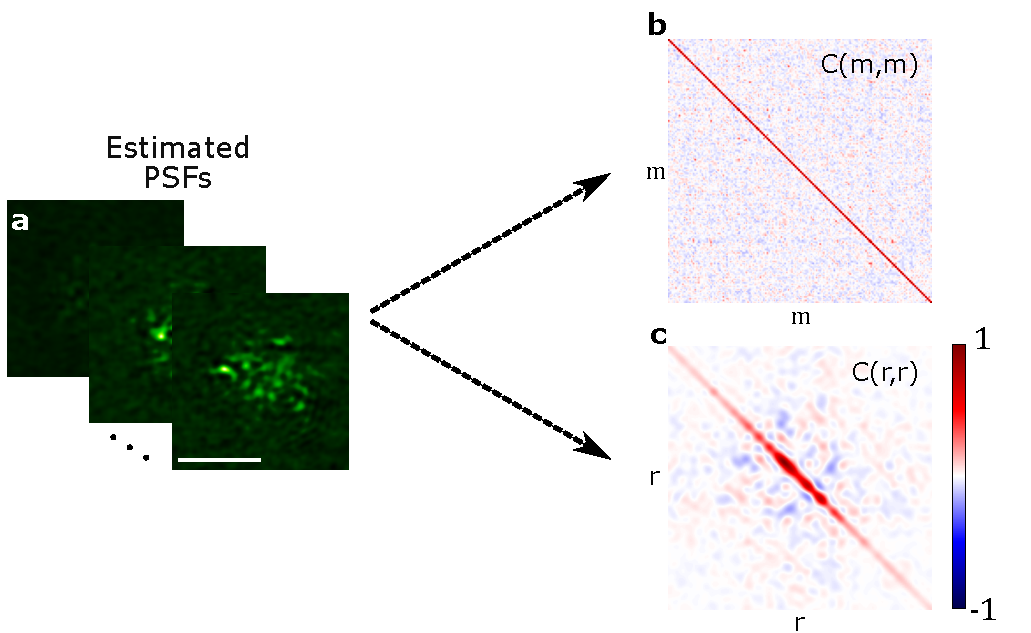
\includegraphics [width=0.98\textwidth,]
	{supp_figures/figure_S1_5.pdf}
         \renewcommand{\thefigure}{S2}

    \caption{\textbf{Verifying the uncorrelation condition of P-matrx}. \textbf{a} the initial estimated PSFs, similar to Fig.~\ref{fig_S1}c, obtained by deconvolving the retrieved object with the captured distorted frames. \textbf{b} displays the frame-wise correlation between different PSFs, and \textbf{c} illustrates the pixel-wise correlation between the estimated PSFs, calculated for the middle camera row due to memory limitations. Here, $M = 150$ and $N = 500^2$. Scale bars, 100 $\mu m$.} 
    \label{fig_S1_5}
    \end{figure} 


Additionally, we provide supplementary videos S1 and S2 that show each frame of \( I_m \) alongside its estimated PSFs. These videos underscore the temporal dynamics in PSF variations and the utility of frame-wise deconvolution in PSF reconstruction.



% %%%%%%%%%%%%%%% Figure s1 - Simulation%%%%%%%%%%%%%%%%%%%%%%
% \begin{figure}[htb!]
% 	\centering
% 	\includegraphics [width=\textwidth,]
% 	{supp_figures/fig1_supp_OLD.pdf}
%          \renewcommand{\thefigure}{S1}

%     \caption{\textbf{Numerical example imaging through dynamic scattering media}. }
%     \label{fig_S3}
% \end{figure} 

\newpage 

\section{Energy conservation as a source of correlation to the PSFs}

A key assumption in our approach is that the PSFs matrix, \textbf{P}, which contains the different time-varying PSFs at its columns, consists of uncorrelated speckle intensity patterns, with a spatial correlation determined by the detection speckle grain size $\delta x$. This assumption results in the covariance matrix of \textbf{P}, being a predominantly diagonal matrix, with off-diagonal correlations extending to $\delta x$ outside the diagonal (Fig.\ref{figS2}a). This diagonal's effective 'width' is dictated by the detection PSF, governed by the illumination numerical aperture (NA) and detection wavelength $\lambda$. 
However, when the PSFs originate from phase-only distortions, they have the same total energy, which leads to residual correlations between the different speckles that compose the PSF: e.g., if one speckle grain is brighter and has more energy, the remaining speckle grains in the PSF must have less energy, and vice versa. The effect is naturally more substantial, and the smaller the number of speckles contained in the PSF.

This fundamental effect introduces off-diagonal spatial correlations in the matrix \textbf{P} (Fig.~\ref{figS2}b), which tend to reduce the quality of the reconstruction, as expected due to the covariance matrix being not diagonal as required for CTR-CLASS \cite{lee22} and I-CLASS \cite{weinberg2023noninvasive}. This is demonstrated in Figure \ref{figS2}c, where the experimental frames of Fig.2b-e, captured through a phase-only diffuser, were processed directly by the I-CLASS algorithm. The reconstructed image (Fig.~\ref{figS2}c) shows the main features of the object on top of a varying hazy, slowly varying background. 
Post-processing can suppress this effect by multiplying each camera frame by a different fixed scalar factor. Thus, PSFs of different total energy are artificially generated. Fig.~\ref{figS2}d shows the reconstruction using the same data as Fig.~\ref{figS2}c but by applying I-CLASS after the scalar multiplication of the captured frames, with multiplication factors linearly varying from 1 to 2 with the frame numbers 1-150. 
Importantly, as expected, this phenomenon only occurs in our experiments that induce stepper motor rotation of a small-angle scattering element, such as the $0.5^\circ$ holographic diffuser in Fig.~2b-m and Fig.~4 of the main text, and not in the experiments that utilize the $1^\circ$ holographic diffuser (Fig.~2n-q), due to the relatively small number of speckles in the PSF in these cases.
%where other experimental measurements did not require this multiplication. This approach effectively de-correlates the PSFs while maintaining the overall structure of the speckle patterns, thus improving our imaging technique's performance.

To visualize the source of the effect of energy conservation on the covariance matrix, we present the covariance matrix of a numerically simulated dynamic scattering matrix \textbf{P}, with and without energy conservation (Fig.~\ref{figS2}a and b, respectively). The impact of energy conservation is evident in the non-negligible (negative) correlations observed in the off-diagonal elements. This is further illustrated by displaying a cross-section of the covariance matrix, showing the negative correlations around the point of interest due to energy conservation. 
%We also provide an example of experimental reconstruction using our proposed intensity modulation technique for energy conservation measurements, similar to those shown in Fig.2 of the main text, utilizing the same optical configuration of widefield transmission incoherent microscopy. (Fig.~\ref{figS2}C and D, respectively) compares the I-CLASS reconstruction without and with the added energy modulation, demonstrating the removal of intensity haze outside the reconstructed target. For completeness, we include several camera frames and an image taken without the scattering, as in Fig.~2 of the main text.

\pagebreak

%%%%%%%%%%%%%%% Figure s2 - Energy consevation%%%%%%%%%%%%%%%%%%%%%%
\begin{figure}[htb!]
	\centering
	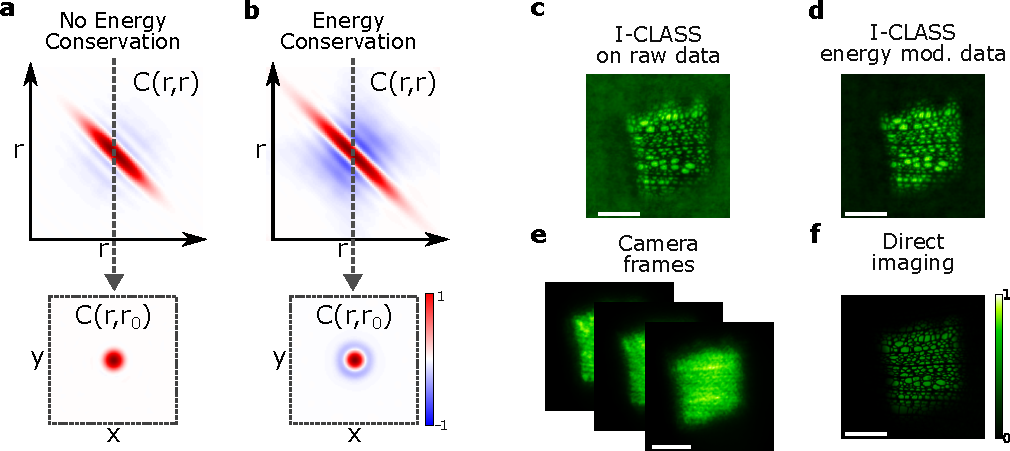
\includegraphics [width=0.98\textwidth,]
	{supp_figures/figure_S2.pdf}
         \renewcommand{\thefigure}{S3}

    \caption{\textbf{Experimental reconstructions under energy conservation}. \textbf{a} The covariance matrix of numerically dynamic scattering matrix \textbf{P}, displayed with and without energy conservation (\textbf{b}). The effect of energy conservation is highlighted by the negative correlation observed in the off-diagonal elements, further illustrated through a cross-section of the covariance matrix. The positive correlation in both cases indicates the influence of finite speckle size. 
    \textbf{c,d} Experimental comparison of I-CLASS reconstructions with and without the application of intensity modulation for energy conservation. The reconstruction with energy modulation shows a reduction of intensity haze outside the reconstructed target. \textbf{e,f} Several camera frames and images taken without the scattering are provided for reference, using the optical setup in Fig.~2 of the main text.}
        \label{figS2}
\end{figure} 

\pagebreak



\section{Comparison with speckle-correlation phase-retrieval based reconstruction}

We present a numerical comparison between our proposed I-CLASS method and the speckle correlation imaging of Katz et al. \cite{katz14}, which is, in essence, equivalent to running a phase-retrieval algorithm on the estimated object autocorrelation (that is, its power spectrum) as originally proposed by Labeyrie's stellar speckle interferometry \cite{labeyrie1970attainment}. %bispectrum-based reconstruction methodology introduced by Wu et al. (24). 
Both methods utilize similar experimental setups and image acquisition schemes, allowing for a direct performance evaluation. To perform this comparison, we focused on several numerically simulated isoplanatic imaging scenarios, demonstrating the superior performance of the matricial I-CLASS approach when reconstructing complex non-sparse natural target objects.

The results of this study are presented in Fig.~\ref{fig_S3} displays a side-by-side comparison between the I-CLASS and speckle correlation reconstruction methods for both sparse and non-sparse objects under two different cases of the number of acquired frames (Figs.~\ref{fig_S3}b,f,j). We numerically simulate camera frames under dynamic scattering by Fourier transforming a random phase mask drawn from a uniform distribution over $[0, 2\pi]$ and taking the squared absolute value. For a very sparse target consisting of two points (Fig.~\ref{fig_S3}a), the speckle correlation imaging (Fig.\ref{fig_S3}c), which uses the Hybrid Input-Output (HIO) algorithm \cite{fienup1978reconstruction} for phase retrieval, shows similar performance to the I-CLASS method, as indicated by the final correlation between the ground-truth image and the reconstructed image (Fig.~\ref{fig_S3}d). However, for more complex simulated objects, such as the Cameraman (Fig.~\ref{fig_S3}e) and a USAF resolution target (Fig.~\ref{fig_S3}i), the speckle correlation reconstruction (Fig.~\ref{fig_S3}g,k) fails to produce results comparable to the I-CLASS method, which demonstrates significantly superior performance (Fig.~\ref{fig_S3}h,l).
\pagebreak

%%%%%Simulation
%%%%%%%%%%%%%%%%%%%%%%
\begin{figure}[hbt!]
	\centering
	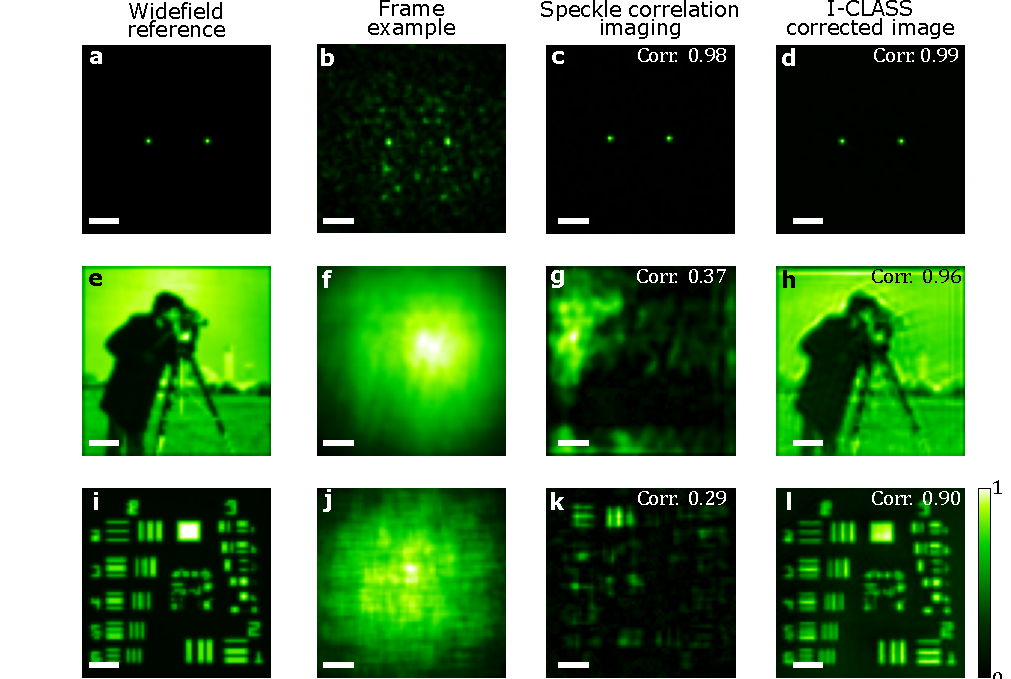
\includegraphics [width=0.98\textwidth,]
	{supp_figures/figure_S3.pdf}
         \renewcommand{\thefigure}{S4}
    \caption{\textbf{Numerical example imaging through dynamic scattering media.} 
    Comparison of the I-CLASS and speckle correlation imaging for both sparse and non-sparse objects. \textbf{a,e,i} Numerically simulated target objects ranging from sparse (two points) to non-sparse targets (Cameraman, USAF resolution target). \textbf{b,f,j} Camera frames simulated under dynamic scattering. \textbf{c,g,k} Speckle correlation imaging successfully reconstructs the sparse target (c) but fails to recover the non-sparse targets (g, k). \textbf{d,h,l} I-CLASS reconstructions demonstrate high fidelity, showing high correlations with the ground-truth images for all simulated objects.  HIO $\beta = 1$, Scale bar: 10 [px]}
        \label{fig_S3}
\end{figure} 



\newpage

\section{Modified CLASS Algorithm (I-CLASS)}
\subsection*{Forward Model}

In the context of incoherent imaging of fluorescence targets through a disordered media, where an object is located within the optical memory effect regime \cite{feng1988correlations}, the image intensity can be described as a convolution of the intensity impulse response (PSF) with the ideal image intensity \cite{goodman2005introduction}.
For coherent illumination of a fluorescence target object, we obtain the following:

\begin{equation}
{I}(\vec{r}) = (|{E}_{in}(\vec{r})*{P}^{(E)}_{ill}(\vec{r})|^2{O}(\vec{r}))*{P}(\vec{r})
\label{eq:1}
\tag{S1}
\end{equation}

Where ${P}^{(E)}_{ill}, {P}_{det}$ are the coherent illumination A-PSF and incoherent detection PSF, respectively, and ${O}(\vec{r})$ is the intensity distribution function of the object.

Thus, under conditions of coherent random illuminations, the fluorescence measurement matrix can be constructed in the spatial basis of variable $\vec{r}$, which is sampled and quantized by the $N$ discrete camera pixels. This construction can be expressed mathematically as follows: ${\textbf{A}} = \textbf{P}_{det}\textbf{O}|\textbf{P}^{(E)}_{ill}\textbf{S}^{(E)}|^2$.
Notably, $\textbf{P}^{(E)}_{ill}$ and $\textbf{P}_{det}$ represent convolution matrices, the optical system input illumination coherent A-PSF and detection incoherent PSF, respectively. Furthermore, the matrix ${\textbf{O}}$ is described by a diagonal matrix, carrying the elements of ${O}(\vec{r})$ on its diagonal, and $\textbf{S}^{(E)}$ contains $M$ columns that represent the $M$ random fields in the illumination plane. For simplicity let us denote the matrix  $\textbf{S} \stackrel{\text{def}} = |\textbf{P}^{(E)}_{ill}\textbf{S}^{(E)}|^2$.

Since $\textbf{S}$ is composed of independent intensity speckle-patterns originating from the same source, one can show that since the patterns are independent, the correlation between a pair of pixels ${a,b}$ and speckle patterns ${i,j}$ can be expressed as $\overline{I_{i_a}I_{j_b}}=\bar{I_a}\bar{I_b}+\delta_{a,b}\delta_{i,j}\bar{I_a}^2$ (using $\overline{I^2}=2\bar{I}^2$) (47).

\noindent This leads to $\overline{(\textbf{S}\textbf{S}^{T})_{i,j}} = \sum^{M-1}_{k=0}\overline{I_{k_i}I_{k_j}} = M\bar{I_i}\bar{I_j}+M\delta_{i,j}\bar{I_i}^2$.

\noindent Thus, considering $\overline{(\textbf{S}\textbf{S}^{T})^2_{i,j}}=\sum^{M-1}_{k,k'=(0,0)}\overline{I_{k_i}I_{k_j}I_{k'_i}I_{k'_j}} = \underbrace{(M^2-M)\overline{I_{i}I_{j}}^2}_{k\neq k'}+M\overline{I^2_{i}I^2_{j}}$ 
and by using $\overline{I^n_i}=n!\overline{I_i}^n$,  it can be demonstrated that:$\frac{\Delta(\textbf{S}\textbf{S}^{T})_{i,j}}{(\textbf{S}\textbf{S}^{T})_{i,j}} \sim \frac{1}{\sqrt{M}}$
(where $\Delta X$ signifies the standard deviation of $X$). 

Consequently, we conclude that to a good approximation $\textbf{S}\textbf{S}^{T} \approx Mdiag(\bar{I}\odot \bar{I}) + M\vec{\bar{I}}\vec{\bar{I}}^T$ where $\vec{\bar{I}}$ is the vector that holds the mean intensity values for each pixel ($\odot$ is the element-wise Hadamard product).
Building on this, we define $\hat{\textbf{S}}\stackrel{\text{def}} = \textbf{S} (\mathbf{I}-\frac{1}{M}\cdot\vec{1}\vec{1}^T)$, where $\vec{1}$ represents a column vector comprising entirely of ones ($\forall i\in[N] :
\vec{1}_{i}=1$) and $\mathbf{I}$ is the identity matrix. This modification effectively normalizes the speckle data by removing the average intensity contribution from each pixel.
Importantly, this transformation renders $\hat{\textbf{S}}$ uncorrelated:

\begin{align}
&\hat{\textbf{S}} \hat{\textbf{S}}^T = \textbf{S}(\mathbf{I}-\frac{1}{M}\cdot\vec{1}\vec{1}^T)^2\textbf{S}^T = \textbf{S}(\mathbf{I}-\frac{1}{M}\cdot\vec{1}\vec{1}^T)\textbf{S}^T \nonumber &\\ &= \textbf{S}\textbf{S}^T-\frac{1}{M}
\underbrace{(\textbf{S}\vec{1})}_{\approx M\vec{\bar{I}}}
\underbrace{(\textbf{S}\vec{1})^T}_{\approx M\vec{\bar{I}}^T}\approx Mdiag(\bar{I}\odot \bar{I}) + M\vec{\bar{I}}\vec{\bar{I}}^T- M\vec{\bar{I}}\vec{\bar{I}}^T = Mdiag(\bar{I}\odot \bar{I}) &
\label{eq:2}
\tag{S2}
\end{align}
leading to the approximation ${\hat{\textbf{S}}} \hat{\textbf{S}}^T \approx \textbf{D}$, for $\textbf{D}\stackrel{\text{def}} =  Mdiag(\bar{I}\odot \bar{I})$.

% We note that this approximation assumes that the spatial autocorrelation of the random speckle pattern is negligible, and can be considered as an additive complex random noise \cite{lee22}, but in fact, as the speckle size is finite, there exists some spatial correlation which smears the object's spectrum \cite{katz14}.

Notably, from a mathematical perspective, it becomes apparent that by subtracting the temporal mean from the measurement matrix $\textbf{A}$, we effectively replicate an illumination pattern with uncorrelated illuminations $\hat{\textbf{S}}$:

\begin{equation}
\hat{\textbf{A}}\stackrel{\text{def}} = {\textbf{A}}(\mathbf{I}-\frac{1}{M}\cdot\vec{1}\vec{1}^T) = {\textbf{P}_{det}}{\textbf{O}}{\textbf{S}}(\mathbf{I}-\frac{1}{M}\cdot\vec{1}\vec{1}^T)
 = {\textbf{P}_{det}}{\textbf{O}}\hat{\textbf{S}}
 \label{eq:3}
\tag{S3}
\end{equation}
From the above calculation of the covariance matrix, we overall get:
\begin{equation}
\textbf{R}_{virt}=\hat{\textbf{A}}\hat{\textbf{A}}^T = {\textbf{P}_{det}}\textbf{O}\hat{\textbf{S}}\hat{\textbf{S}}^T\textbf{O}\textbf{P}_{det}^T \approx \textbf{P}_{det}{\textbf{O}_{eff}} \textbf{P}_{det}^T
\tag{S4}
\label{eq:4}
\end{equation}
For $\textbf{O}_{eff}\stackrel{\text{def}}=\textbf{O}^2 \textbf{D}$, an incoherent fluorescent analog to a virtual reflection matrix.
Utilizing the multiplication-convolution relationship in $\vec{k}$-space, we can decompose the Fourier transform of the reflection matrix into: 
\begin{align}
\tag{S5}
\label{eq:5}
\tilde{\textbf{R}}_{virt}\equiv\mathcal{F}\textbf{R}_{virt}\mathcal{F}^{\dagger} \approx  \mathcal{F}\textbf{P}_{det}{\textbf{O}_{eff}} \textbf{P}_{det}^T\mathcal{F}^{\dagger} = &&  \\ \nonumber 
\mathcal{F}\textbf{P}_{det}\mathcal{F}^{\dagger}\mathcal{F}\textbf{O}_{eff}\mathcal{F}^{\dagger}(\mathcal{F}\textbf{P}_{det}\mathcal{F}^{\dagger})^{\dagger}={\tilde{\textbf{P}}_{det}}{\tilde{\textbf{O}}_{eff}}{\tilde{\textbf{P}}^{\dagger}_{det}}
\end{align}
(where $\mathcal{F}$ represents the unitary DFT matrix).


In this Fourier domain representation, $\tilde{\textbf{P}}_{det}$ which is the Fourier transform of $\textbf{P}_{det}$, takes on a diagonal form, reflecting the fact that the convolution operations in real space become simple multiplications in Fourier space. In the case of a unitary phase-only distortion (which is the model in the coherent case), these diagonal matrices contain the random phases $e^{i\phi_{det}(\vec{k})}$ and $e^{-i\phi_{det}(\vec{k})}$, respectively, which the CLASS algorithm aims to correct. On the other hand, the matrix $\tilde{\textbf{O}}_{eff}$ which is the Fourier transform of $\textbf{O}_{eff}$, now adopts the form of a Toeplitz convolution matrix, with the Fourier components of the object.

\subsection*{CLASS algorithm}

The CLASS algorithm \cite{kang17} aims to correct the distortion, $\tilde{\textbf{P}}_{det}$, and retrieve the ideal image intensity ${\tilde{\textbf{O}}_{eff}}$. Mathematically, this requires finding the inverse of $\tilde{\textbf{P}}_{det}$ which, being modeled as a unitary transformation with only phase aberrations, is equivalent to finding $\tilde{\textbf{P}}_{det}^{\dagger}$.
We note that very recently, a tutorial with detailed algorithm implementations of CLASS was published \cite{kang2024implementation}. 
%The algorithm aims to minimize the difference between the k-space $\tilde{\textbf{R}}$ and $\tilde{\textbf{P}}_{det}^{\dagger}\tilde{\textbf{P}}_{det}\tilde{\textbf{O}}_{eff}\tilde{\textbf{P}}_{det}^{\dagger}\tilde{\textbf{P}}_{det} = \tilde{\textbf{O}}_{eff}$, which is a Toeplitz matrix. 
% The second perspective involves maximizing the diagonal elements of $\textbf{R}$ in $r$-space, which represent the "effective confocal energy". Both perspectives are entirely equivalent, as evidenced by their Fourier relations.
%The problem is addressed in k-space in the CLASS algorithm, where $\tilde{\textbf{P}}_{det}$ is modeled as a diagonal matrix containing only phase components on its diagonal.

The standard CLASS algorithm, handling a full system reflection matrix in the form of  $\textbf{R}={\tilde{\textbf{P}}_{det}}{\tilde{\textbf{O}}}{\tilde{\textbf{P}}_{ill}}$, addresses a single distortion during each iteration, alternately handling $\tilde{\textbf{P}}_{det}$ and $\tilde{\textbf{P}}_{ill}$. However, in CTR-CLASS \cite{lee22} where $\tilde{\textbf{P}}_{ill} = \tilde{\textbf{P}}_{det}$, exclusively tackles the "right" matrix $\tilde{\textbf{P}}_{det}$ in each iteration and fixes the matrix from both sides.

In each iteration of the CLASS algorithm, only a single aberration is corrected—either the output (detection) or the input (illumination) aberration. Specifically, when correcting the input aberration, the output aberration is temporarily neglected, and vice versa. The convergence of CLASS assumes correlation in the uncorrected aberration in each iteration \cite{kang17}. Therefore if we displace each column proportionally to its index, the resultant matrix should approximately exhibit columns of equal values which contain the spectrum of $\tilde{O}_{eff}(\vec{k})$, albeit with distinct global phases for each column. Consequently, if we compute the average of these columns, we obtain a reasonably accurate estimation of $\tilde{O}_{eff}(\vec{k})$, given that the phase averages out.\\
Now that we possess an approximation of $\tilde{O}_{eff}(\vec{k})$, we can determine the overall phase for each column. This can be achieved by calculating the correlation angle between the j-th column and the estimated $\hat{\tilde{O}}_{eff}(\vec{k})$:

\begin{equation}
\hat{\phi}_{det}({k_{j})} = arg\{<\hat{\tilde{O}}_{eff}^*(\vec{k})\tilde{O}_{eff}(\vec{k})e^{i\phi_{det}(k_{j})}>_k\}
\tag{S6}
\label{eq:6}
\end{equation}
By incorporating the terms $e^{-i\hat{\phi}_{det}(\vec{k})}$ into a diagonal matrix $\hat{\tilde{\textbf{P}}}_{det}$ we can fix $\tilde{\textbf{R}}$ by $\tilde{\textbf{R}}_t=\hat{\tilde{\textbf{P}}}_{det}^{\dagger}\tilde{\textbf{R}}_{t-1}\hat{\tilde{\textbf{P}}}_{det}$. This iterative approach consistently leads to the convergence of the correct phase correction.
We now write the iteration in a matrix notation by defining the following:
\begin{equation}
\vec{z}\stackrel{\text{def}} =  \tilde{\textbf{R}}^{T}_{n_s}(\tilde{\textbf{R}}_{n_s}\vec{1})^*=(\tilde{\textbf{R}}^{\dagger}_{n_s}\tilde{\textbf{R}}_{n_s}\vec{1})^*=\vec{1}^T\tilde{\textbf{R}}^{\dagger}_{n_s}\tilde{\textbf{R}}_{n_s}
\tag{S7}
\label{eq:7}
\end{equation}

With this notation, we obtain:  $\hat{\phi}_{det}({k_{j})}=\frac{\vec{z}_j}{|\vec{z}_j|}$

Here, $\tilde{\textbf{R}}_{n_s}$ represents the shifted version of $\tilde{\textbf{R}}^{(ud)}$, which can be expressed as:
\begin{equation}
\forall i\in[2N-1] \forall j\in[N]:
\tilde{\textbf{R}}_{n_{s_{i,j}}}=\sum^{N-1}_{a=0}\sum^{N-1}_{b=0}S_{i,j,a,b}\tilde{\textbf{R}}^{(ud)}_{n_{a,b}}
\tag{S8}
\label{eq:8}
\end{equation}
Using $S_{i,j,a,b} = \delta_{j,b}\delta_{i,a+b}$, where $N$ represents the camera pixel count. Additionally, we use $\tilde{\textbf{R}}^{(ud)}_{n_{i,j}} = \tilde{\textbf{R}}_{N-1-i,j}$ i.e. flipping each column of $\tilde{\textbf{R}}$, a measure that was taken for the sake of index convenience.
(By denoting $\textbf{R}^{(ud)}_{{i,j}} = \textbf{R}_{N-1-i,j}$ we can get $\tilde{\textbf{R}}^{(ud)} = \tilde{\textbf{A}}^{(ud)}\tilde{\textbf{A}}^\dagger$)
% 



\subsection*{Memory Complexity}
Given that we capture only $M$ images from distinct random illuminations, each containing $N$ pixels, where $M<<N$, it is advantageous to avoid explicitly constructing the matrix $\textbf{R}_{virt}$ as ${\hat{\textbf{A}}}{\hat{\textbf{A}}}^{\dagger}$, an $N$x$N$, matrix, due to its high memory demand. All the necessary information should be encapsulated within $\hat{\textbf{A}}$, which is of size $N$x$M$. As a result, we show an equivalent mathematical expression for a CLASS iteration using $\hat{\textbf{A}}$ without directly computing $\textbf{R}_{virt}$.

We note that since the DFT matrix \( \mathcal{F} \) is unitary, we can apply a two-dimensional Fourier transform to the measured images before including them in \( {\hat{\textbf{A}}} \), thus obtaining \( \tilde{\textbf{R}}_{virt} = \mathcal{F}\textbf{R}_{virt}\mathcal{F}^{\dagger} = \mathcal{F}{\hat{\textbf{A}}}{\hat{\textbf{A}}}^{\dagger}\mathcal{F}^{\dagger} = \mathcal{F}{\hat{\textbf{A}}}\mathcal{F}^T(\mathcal{F}{\hat{\textbf{A}}}\mathcal{F}^T)^{\dagger} \). Therefore, we can concentrate on $\tilde{\textbf{A}}=\mathcal{F}{\hat{\textbf{A}}}\mathcal{F}^{T}$.

First, we find the vector elements of $\vec{z} = \vec{1}^T\tilde{\textbf{R}}^{\dagger}_{n_s}\tilde{\textbf{R}}_{n_s}$ (Eq.~\ref{eq:7}):

\begin{align}
& z_j = \sum^{N-1}_{i=0}(\tilde{\textbf{R}}^{\dagger}_{s}\tilde{\textbf{R}}_{s})_{i,j} = \sum^{N-1}_{i=0} \sum^{2N-2}_{m=0}(\tilde{\textbf{R}}^{*}_{s_{m,i}}\tilde{\textbf{R}}_{s_{m,j}}) \nonumber &\\&\underset{(S8)}{=}  \sum^{N-1}_{i=0}\sum^{2N-2}_{m=0}\sum^{N-1}_{k=0}\sum^{N-1}_{l=0}\sum^{N-1}_{a=0}\sum^{N-1}_{b=0}S_{m,j,a,b}\tilde{\textbf{R}}^{(ud)}_{a,b}S_{m,i,k,l}\tilde{\textbf{R}}^{(ud)^*}_{k,l} \nonumber &\\ 
&= \sum^{N-1}_{i=0}\sum^{N-1}_{k=0}\sum^{N-1}_{l=0}\sum^{N-1}_{a=0}\sum^{N-1}_{b=0}\tilde{\textbf{R}}^{(ud)^*}_{k,l}\tilde{\textbf{R}}^{(ud)}_{a,b}\sum^{2N-2}_{m=0}S_{m,j,a,b}S_{m,i,k,l} \nonumber &\\ 
&= \sum^{N-1}_{i=0}\sum^{N-1}_{k=0}\sum^{N-1}_{l=0}\sum^{N-1}_{a=0}\sum^{N-1}_{b=0}\tilde{\textbf{R}}^{(ud)^*}_{k,l}\tilde{\textbf{R}}^{(ud)}_{a,b}\delta_{j,b}\delta_{i,l}\sum^{2N-2}_{m=0}\delta_{m,a+b}\delta_{m,k+l} \nonumber &\\ 
&= (2N-1)\sum^{N-1}_{i=0}\sum^{N-1}_{k=0}\sum^{N-1}_{a=0}\tilde{\textbf{R}}^{(ud)}_{a,j}\tilde{\textbf{R}}^{(ud)^*}_{k,i}\delta_{a+j,k+i} \nonumber &\\ 
&\propto \sum^{N-1}_{i=0}\sum^{N-1}_{k=0}\sum^{N-1}_{a=0}\sum^{M-1}_{n=0}\sum^{M-1}_{m=0}\tilde{\textbf{A}}^{(ud)}_{a,n}\tilde{\textbf{A}}^*_{j,n}\tilde{\textbf{A}}^{(ud)^*}_{k,m}\tilde{\textbf{A}}_{i,m}\delta_{a+j,k+i} \nonumber &\\ 
&= \sum^{N-1}_{k=0}\sum^{N-1}_{a=0}\sum^{M-1}_{n=0}\tilde{\textbf{A}}^{(ud)}_{a,n}\tilde{\textbf{A}}^*_{j,n}\sum^{M-1}_{m=0}\tilde{\textbf{A}}^{(ud)^*}_{k,m}\tilde{\textbf{A}}_{a+j-k,m}\sum^{N-1}_{i=0}\delta_{a+j,k+i}
 \nonumber &\\ 
&= \sum^{N-1}_{a=0}\langle \vec{\tilde{\textbf{A}}}_{j,:},\vec{\tilde{\textbf{A}}}^{(ud)}_{a,:} \rangle\sum^{min(N-1,a+j)}_{k=max(0,a+j-(N-1))}\langle \vec{\tilde{\textbf{A}}}^{(ud)}_{k,:},\vec{\tilde{\textbf{A}}}_{a+j-k,:} \rangle &
\tag{S9}
\label{eq:9}
\end{align}

where we denote $\vec{\tilde{\textbf{A}}}_{c,:}$ as the c-th column of $\tilde{\textbf{A}}$. By denoting ${\textbf{A}}^{(lr)}_{a,b}={\textbf{A}}_{a,M-1-b}$ and using full-sized convolution (with zero-padding) yields:
\begin{equation}
({\textbf{A}}^{(ud)^*}*{\textbf{A}}^{(lr)})_{a+j,M-1} = \sum^{min(N-1,a+j)}_{k=max(0,a+j-(N-1))}\langle {\textbf{A}}^{(ud)}_{k,:},{\textbf{A}}_{a+j-k,:} \rangle \label{eq:10} \tag{S10}
\end{equation}
By plugging Eq.~\ref{eq:10} into Eq.~\ref{eq:9}, we obtain:

\begin{equation}
\vec{z}=\sum^{N-1}_{a=0}(\tilde{\textbf{A}}^*\vec{\tilde{\textbf{A}}}_{a,:})\odot(\tilde{\textbf{A}}^{(ud)^*}*\tilde{\textbf{A}}^{(lr)})_{a:a+N,M-1}
\label{eq:11} \tag{S11}
\end{equation}
Where $\odot$ denotes the Hadamard Product (element-wise multiplication) between two vectors. And the phase correction for each iteration is received by $\hat{\vec{\phi}} = \frac{\vec{z}}{|\vec{z}|}$ (element-wise division).

To furtherly remove the sum over $a$, we denote $\vec{b}\stackrel{\text{def}} = (\tilde{\textbf{A}}^{(ud)^*}*\tilde{\textbf{A}}^{(lr)})_{:,M-1}$, rewriting the expression of $\vec{z}$ as:

\begin{equation}
z_i=(\sum^{N-1}_{a=0}(\tilde{\textbf{A}}^*\vec{\tilde{\textbf{A}}}_{a,:})\odot\vec{b}_{a:a+N})_i =\sum^{M-1}_{j=0} \tilde{\textbf{A}}^*_{i,j}\sum^{N-1}_{a=0}\tilde{\textbf{A}}^{(ud)}_{a,j}\vec{b}_{a+i}=\sum^{M-1}_{j=0} \tilde{\textbf{A}}^*_{i,j}(\vec{b} \star \tilde{\textbf{A}}^{(ud)})_{i,j}
\label{eq:12}  \tag{S12}
\end{equation}
where $\star$ is a 2D cross-correlation.
Finally, the correction can be written simply as:
\begin{equation}
\vec{z}_{t+1}=(\tilde{\textbf{A}}_t^* \odot ((\tilde{\textbf{A}}_t^{(ud)^*}*\tilde{\textbf{A}}_t^{(lr)})_{:,M-1} \star \tilde{\textbf{A}}_t^{(ud)}))\vec{1}
\label{eq:13}  \tag{S13}
\end{equation}
Therefore, after each iteration $t = 1...T$, we update the matrix using the formula
$\tilde{\textbf{A}}_{t+1}=diag\{\frac{\vec{z}_{t+1}}{|\vec{z}_{t+1}|}\}\tilde{\textbf{A}}_t$, where both the exponential function and the division are applied element-wise  (the function $diag\{\vec{x}\}$ constructs a diagonal matrix with the elements of vector $\vec{x}$ placed along its diagonal).
Since building this correction diagonal matrix is memory inefficient, we correct each q-th column of $\tilde{\textbf{A}}_t$ with the element-wise multiplication: $ \frac{\vec{z}_{t+1}}{|\vec{z}_{t+1}|} \odot \tilde{\textbf{A}}_{t_{:,q}}$.

After all iterations, to restore the object approximation $\hat{O}_{eff}=diag\{\textbf{R}_{virt}\}$ we then calculate:
\begin{align}
\label{eq:14}  \tag{S14}
&\hat{O}_{eff_i}=\textbf{R}_{virt_{i,i}}=\mathcal{F}^{\dagger}\tilde{\textbf{R}}_{virt}\mathcal{F}_{i,i}=\mathcal{F}^{\dagger}\tilde{\textbf{A}}\tilde{\textbf{A}}^\dagger\mathcal{F}_{i,i} &\\ 
&= \mathcal{F}^{\dagger}\tilde{\textbf{A}}\mathcal{F}\mathcal{F}^{\dagger}\tilde{\textbf{A}}^\dagger\mathcal{F}_{i,i} \nonumber = \sum^{N-1}_{m=0}|\mathcal{F}^{\dagger}\tilde{\textbf{A}}\mathcal{F}|^2_{i,m} &
\end{align}
Overall, the object can be written as: $\vec{{O}}_{eff} =|iFFT2(\tilde{\textbf{A}})|^2\vec{1}$, which is the sum over the columns of $|{\hat{\textbf{A}}}|^2$.
We conclude that the improvement in the memory-efficient I-CLASS algorithm now has memory complexity $O(MN)$ instead of $O(N^2)$, an improvement of $N/M$, which in our experiments is $\sim$ $10^4$.







\subsection*{Regularized Fourier Reweighting}

In the incoherent imaging scenario mentioned in the main text, non-unitary distortion and amplitude modulation cause 'haze' in the phase-corrected image. Thus, in estimating the Modulation Transfer Function (MTF), the absolute value of the Optical Transfer Function (OTF), is essential. 

In the preceding discussion, and as demonstrated in Eq.~\ref{eq:5}, we observe that ${\tilde{\textbf{P}}_{det}}$ is structured as a diagonal matrix containing on its diagonal  ${\tilde{\textbf{P}}_{det_{i,i}}}=MTF(k_i)e^{i\phi_{det}(k_i)}$, while ${\tilde{\textbf{O}}_{eff}}$ takes the form of a convolution matrix. This allows us to express the elements of $\tilde{\textbf{R}}$ as follows:

\begin{equation}
\tilde{\textbf{R}}_{i,j} = \sum_{a,b}{\tilde{\textbf{P}}_{det_{i,a}}} \tilde{\textbf{O}}_{eff_{a,b}}{\tilde{\textbf{P}}^{\dagger}_{det_{b,j}}}=\sum_{a,b}{\tilde{\textbf{P}}_{det_{i,i}}} \delta_{i,a} \vec{\tilde{O}}_{eff_{a-b}}{\tilde{\textbf{P}}^*_{det_{j,j}}} \delta_{b,j}
\label{eq:15}  \tag{S15}
\end{equation}
This formulation leads to the following expression for the diagonal elements:

\begin{equation}
\tilde{\textbf{R}}_{i,i} = \vec{\tilde{O}}(0) {\tilde{\textbf{P}}_{det_{i,i}}}{\tilde{\textbf{P}}^*_{det_{i,i}}} \propto |{\tilde{\textbf{P}}_{det_{i,i}}}|^2
\label{eq:16}  \tag{S16}
\end{equation}
Consequently, this relationship enables the estimation of the MTF up to a scaling factor, by:
$\widehat{MTF} \equiv \sqrt{diag\{\tilde{\textbf{R}}\}}$. %We note that this scaling factor limits the quantitative reconstruction. 
Similarly to the approach outlined in Eq.~\ref{eq:14}, the MTF can be directly computed from $\tilde{\textbf{A}}$, bypassing the need for explicit calculation of $\tilde{\textbf{R}}$. This is achieved by summing over the columns of $|{\tilde{\textbf{A}}}|^2$.

This can also be derived in an integral form, which is perhaps more natural for describing the forward optical physical model. Given the forward model \ref{eq:1}  $I_{m}(\vec{r}) = P(\vec{r'}) * (O(\vec{r'}) \cdot S_{m}(\vec{r'}))|_{\vec{r}}$ where $O(\vec{r})$ is the fluorophore distribution (the object function) and $S_{m}(\vec{r})$ is the illumination speckle pattern on the object plane. When assuming, as mentioned above, a delta-like speckle covariance: $C_S(\vec{r}_1,\vec{r}_2) \stackrel{\text{def}} = \langle S_m(\vec{r}_1)S_m(\vec{r}_2) \rangle_m - \langle S_m(\vec{r}_1) \rangle_m \langle S_m(\vec{r}_2) \rangle_m \propto\delta(\vec{r}_1-\vec{r}_2)$, and defining $\hat{S}_m(\vec{r})=S_m(\vec{r})-\langle S_{m'}(\vec{r})\rangle_{m'}$, we obtain $\langle \hat{S}_m(\vec{r}_1)\hat{S}_m(\vec{r}_2) \rangle_m =C_S(\vec{r}_1,\vec{r}_2) \propto\delta(\vec{r}_1-\vec{r}_2)$. Additionally, by defining $\tilde{\hat{I}}_m(\vec{r})\stackrel{\text{def}} = I_m(\vec{r})-\langle I_{m'}(\vec{r})\rangle_{m'}=P(\vec{r'}) * (O(\vec{r'}) \cdot (S_{m}(\vec{r'})-\langle S_{m'}(\vec{r})\rangle_{m'}))=P (\vec{r'})* (O(\vec{r'}) \cdot \hat{S}_{m}(\vec{r'}))|_{\vec{r}}$, we can apply the multiplication-convolution property of the Fourier transform to get: $\tilde{\hat{I}}_m(\vec{k})\stackrel{\text{def}} = OTF(\vec{k})\cdot(\tilde{O}(\vec{k})*\tilde{\hat{S}}_m(\vec{k}))$. Therefore, the spectrum covariance can be expressed as:
\begin{flalign}
&C_I(\vec{k}_1,\vec{k}_2) \stackrel{\text{def}} =  \langle \tilde{\hat{I}}_m(\vec{k}_1)\tilde{\hat{I}}^*_m(\vec{k}_2)   \rangle_m  \nonumber \\& =  
\langle (OTF(\vec{k}_1)\cdot(\tilde{O}(\vec{k}_1)*\tilde{\hat{S}}_m(\vec{k}_1))(OTF(\vec{k}_2)\cdot(\tilde{O}(\vec{k}_2)*\tilde{\hat{S}}_m(\vec{k}_2)))^* \rangle_m \nonumber  \\& =\langle OTF(\vec{k}_1)OTF^*(\vec{k}_2)(\tilde{O}(\vec{k}_1)*\tilde{\hat{S}}_m(\vec{k}_1))\cdot(\tilde{O}^*(\vec{k}_2)*\tilde{\hat{S}}^*_m(\vec{k}_2)) \rangle_m \nonumber  \\& =\langle OTF(\vec{k}_1)OTF^*(\vec{k}_2)\iint\tilde{O} (\vec{k}'-\vec{k}_1)\tilde{\hat{S}}_m(\vec{k}')d\vec{k}'\iint\tilde{O}^* (\vec{k}''-\vec{k}_2)\tilde{\hat{S}}^*_m(\vec{k}'')d\vec{k}'' \rangle_m  \nonumber  \\& =OTF(\vec{k}_1)OTF^*(\vec{k}_2)\iint\tilde{O} (\vec{k}'-\vec{k}_1)d\vec{k}'\iint\tilde{O}^* (\vec{k}''-\vec{k}_2) \nonumber  \\& \iiiint e^{-i\vec{k}'\cdot \vec{r}'}e^{i\vec{k}''\cdot \vec{r}''}\underbrace{\langle{\hat{S}_m(\vec{r}')}{\hat{S}_m(\vec{r}'')}}_{\delta(\vec{r}'-\vec{r}'' )}\rangle_md\vec{k}''d\vec{r}'d\vec{r}'' \nonumber  \\&= OTF(\vec{k}_1)OTF^*(\vec{k}_2)\iint\tilde{O} (\vec{k}'-\vec{k}_1)d\vec{k}'\iint\tilde{O}^* (\vec{k}''-\vec{k}_2) 
d\vec{k}''\underbrace{\iint e^{-i(\vec{k}'-\vec{k}'')\cdot \vec{r}'}d\vec{r}'}_{\delta(\vec{k}'-\vec{k}'')} \nonumber  \\&= OTF(\vec{k}_1)OTF^*(\vec{k}_2)\iint\tilde{O} (\vec{k}'-\vec{k}_1)\tilde{O}^* (\vec{k}'-\vec{k}_2)d\vec{k}'\nonumber  \\&= OTF(\vec{k}_1)OTF^*(\vec{k}_2)\iint\tilde{O} (\vec{k}'')\tilde{O}^* (\vec{k}''+\vec{k}_1-\vec{k}_2)d\vec{k}'' 
\label{eq:17}  \tag{S17}
\end{flalign}
Thus, similarly to Eq. \ref{eq:16}, we obtain on the 'diagonal' of the covariance term:
$C_I(\vec{k},\vec{k}) = |OTF(\vec{k})|^2\iint
|\tilde{O} (\vec{k}'')
|^2d\vec{k}''\propto |OTF(\vec{k})|^2$, and estimate the MTF by $\widehat{MTF}(\vec{k})\equiv\sqrt{C_I(\vec{k},\vec{k})}$


Overall, the $\vec{k}$-space amplitude correction is estimated by taking the amplitude correction $\widehat{MTF}$ as input for a regularized Fourier reweighting process, where each camera frame is reweighted independently with the same amplitude correction. %Fourier component of $\vec{{O}}_{CLASS}$, denoted as  $\vec{\tilde{O}}_{CLASS}$, is divided by a factor given by:
%\begin{equation}
%\vec{\tilde{O}}_{I-CLASS_{i}} \equiv \frac{ \vec{\tilde{O}}_{CLASS_{i}}}{\frac{\widehat{MTF}_i}{\max_{q} \widehat{MTF}_q }+\sigma}
%\label{eq:17}   \tag{S17}
%\end{equation}
\begin{equation}
\tilde{\textbf{A}}_{fixed}=\frac{\tilde{\textbf{A}}_T}{\widehat{MTF}+\sigma}
\label{eq:18}   \tag{S18}
\end{equation}

\noindent where $\sigma$ is the regularization parameter, and $\tilde{\textbf{A}}_T$ are the phase-corrected frames.
Although one can utilize various deconvolution methods, such as Wiener or Richardson-Lucy, our empirical observations have shown that regularized deconvolution yields superior results using the regularization of Eq.\ref{eq:18}.

The impact of different regularization parameters is demonstrated through I-CLASS corrections in Fig.~\ref{fig1_supp}. Fig.~\ref{fig1_supp}A features the CLASS correction, similar to taking the regularization parameter $\sigma $ to $\infty$. Fig.~\ref{fig1_supp}B displays the result of an excessively high regularization parameter, leading to haze in the image. Fig.~\ref{fig1_supp}C demonstrates an optimal balance between noise reduction and the preservation of high-frequency details. Lastly, Fig.~\ref{fig1_supp}D presents the effect of setting the regularization parameter too low, resulting in the inclusion of noisy high-frequency bands.

\begin{figure}[ht!]
	\centering
	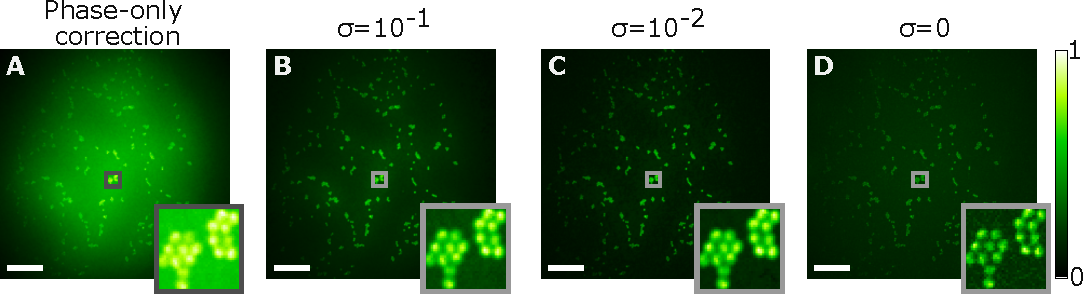
\includegraphics [width=0.98\textwidth,]
	{supp_figures/figure_S5.pdf}
        \renewcommand{\thefigure}{S5}
    \caption{\textbf{Regularized Fourier-reweighting with varying regularization parameter}. (A) Corrected confocal image via phase-only OTF correction shows substantial hazing due to uncorrected amplitude attenuation. (B) The result of a too-high regularization parameter resulted in the inclusion of haze. (C) Shows the scenario where the regularization parameter optimally reduces noise while preserving high-frequency details. (D) Illustrates the effect when the regularization parameter (sigma) is set too low, including noisy high-frequency bands. Scale bars, 200 $\mu m$. Insets in (A-D) compare the marked square areas.}\label{fig1_supp}
\end{figure} 
\noindent In summary, the I-CLASS algorithm proceeds as follows: First, it applies the memory-efficient version of the CTR-CLASS phase correction to all camera frames. Next, it estimates the MTF from the diagonal of the Fourier-transformed reflection matrix. Then, it performs Fourier-reweighting on all camera frames using the estimated MTF. Lastly, it calculates the square root of the variance of the corrected frames, which is the final I-CLASS corrected image.
% In summary, the I-CLASS algorithm proceeds as follows in three steps: initially, it employs the memory-efficient version of the CTR-CLASS phase correction on all camera frames, followed by estimating the MTF from the diagonal of the Fourier-transformed reflection matrix applying deconvolution with the estimated MTF on all camera frames and finally calculating the square root of the variance image.

\newpage

\section*{Digital Autofocus through Fresnel Propagation}
            
    In holographic imaging through scattering media, a key advantage is the ability to numerically propagate the reconstructed complex field to any desired axial plane once the field is retrieved at a single reference plane. This capability, often called digital autofocus, eliminates the necessity of knowing the exact object distance during data acquisition.
    
    In our experiments from Fig.~5 of the main text, the I-CLASS algorithm reconstructs the complex wavefront at the scattering layer plane (z = 0). However, as shown in Fig.~\ref{fig:autofocus}, this field can be digitally propagated to any desired plane using the Fresnel propagation operator described in the Methods section of the main text. 
    
    By computationally varying the propagation distance and observing the resulting reconstructed intensity distributions, we can identify the optimal object plane where the finest features of the target come into focus. This process is analogous to the physical process of adjusting the focus in a conventional microscope, but performed entirely in post-processing.
    
    Figure~S6 demonstrates this capability by showing the reconstructed field intensity at three distinct propagation distances: before the object plane (z = 5.3 cm), at the object plane where optimal focus is achieved (z = 7.15 cm), and after the object plane (z = 9 cm). The sharp focus observed at z = 7.15 cm confirms that this is indeed the correct object plane, with clear resolution of the fine features in the USAF target.

    \begin{figure}[hb]
        \centering
        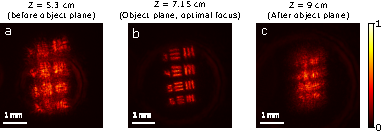
\includegraphics[width=0.99\textwidth]{supp_figures/figure_S6.pdf}
        \caption{\textbf{Digital autofocus capability through numerical propagation of the reconstructed complex field.} The reconstructed field intensity is shown at three different propagation distances: \textbf{a} z = 5.3 cm (before the object plane), \textbf{b} z = 7.15 cm (at the object plane, where optimal focus is achieved), and \textbf{c} z = 9.0 cm (after the object plane). The sharp focus visible in panel \textbf{b} confirms the correct object plane location, demonstrating that precise knowledge of the object-diffuser distance is not required during data acquisition as optimal focus can be determined computationally during post-processing. Scale bars: 1 mm.}
            \label{fig:autofocus}

    \end{figure}

           

\newpage

\section*{Effect of illumination spot size on coherent imaging through dynamic scattering}

In our coherent imaging configuration (Fig. 5 of the main text), maintaining a constant illumination pattern at the object plane despite the dynamic scattering introduced by the rotating diffuser is crucial for successful application of our reconstruction algorithm. As expressed in Eq. 6-7 of the main text, our method requires that the illumination field $E_m^{ill}(\vec{r})$ remains effectively constant across different acquisitions for our method to work properly.

This requirement might appear contradictory, as one might expect that any illumination passing through a dynamic scatterer would inevitably result in varying illumination patterns. However, the key insight is that the relationship between the illumination spot size on the diffuser and the diffuser's correlation length determines whether the illumination at the object plane remains approximately constant between different diffuser realizations.

\begin{figure}
	\centering
	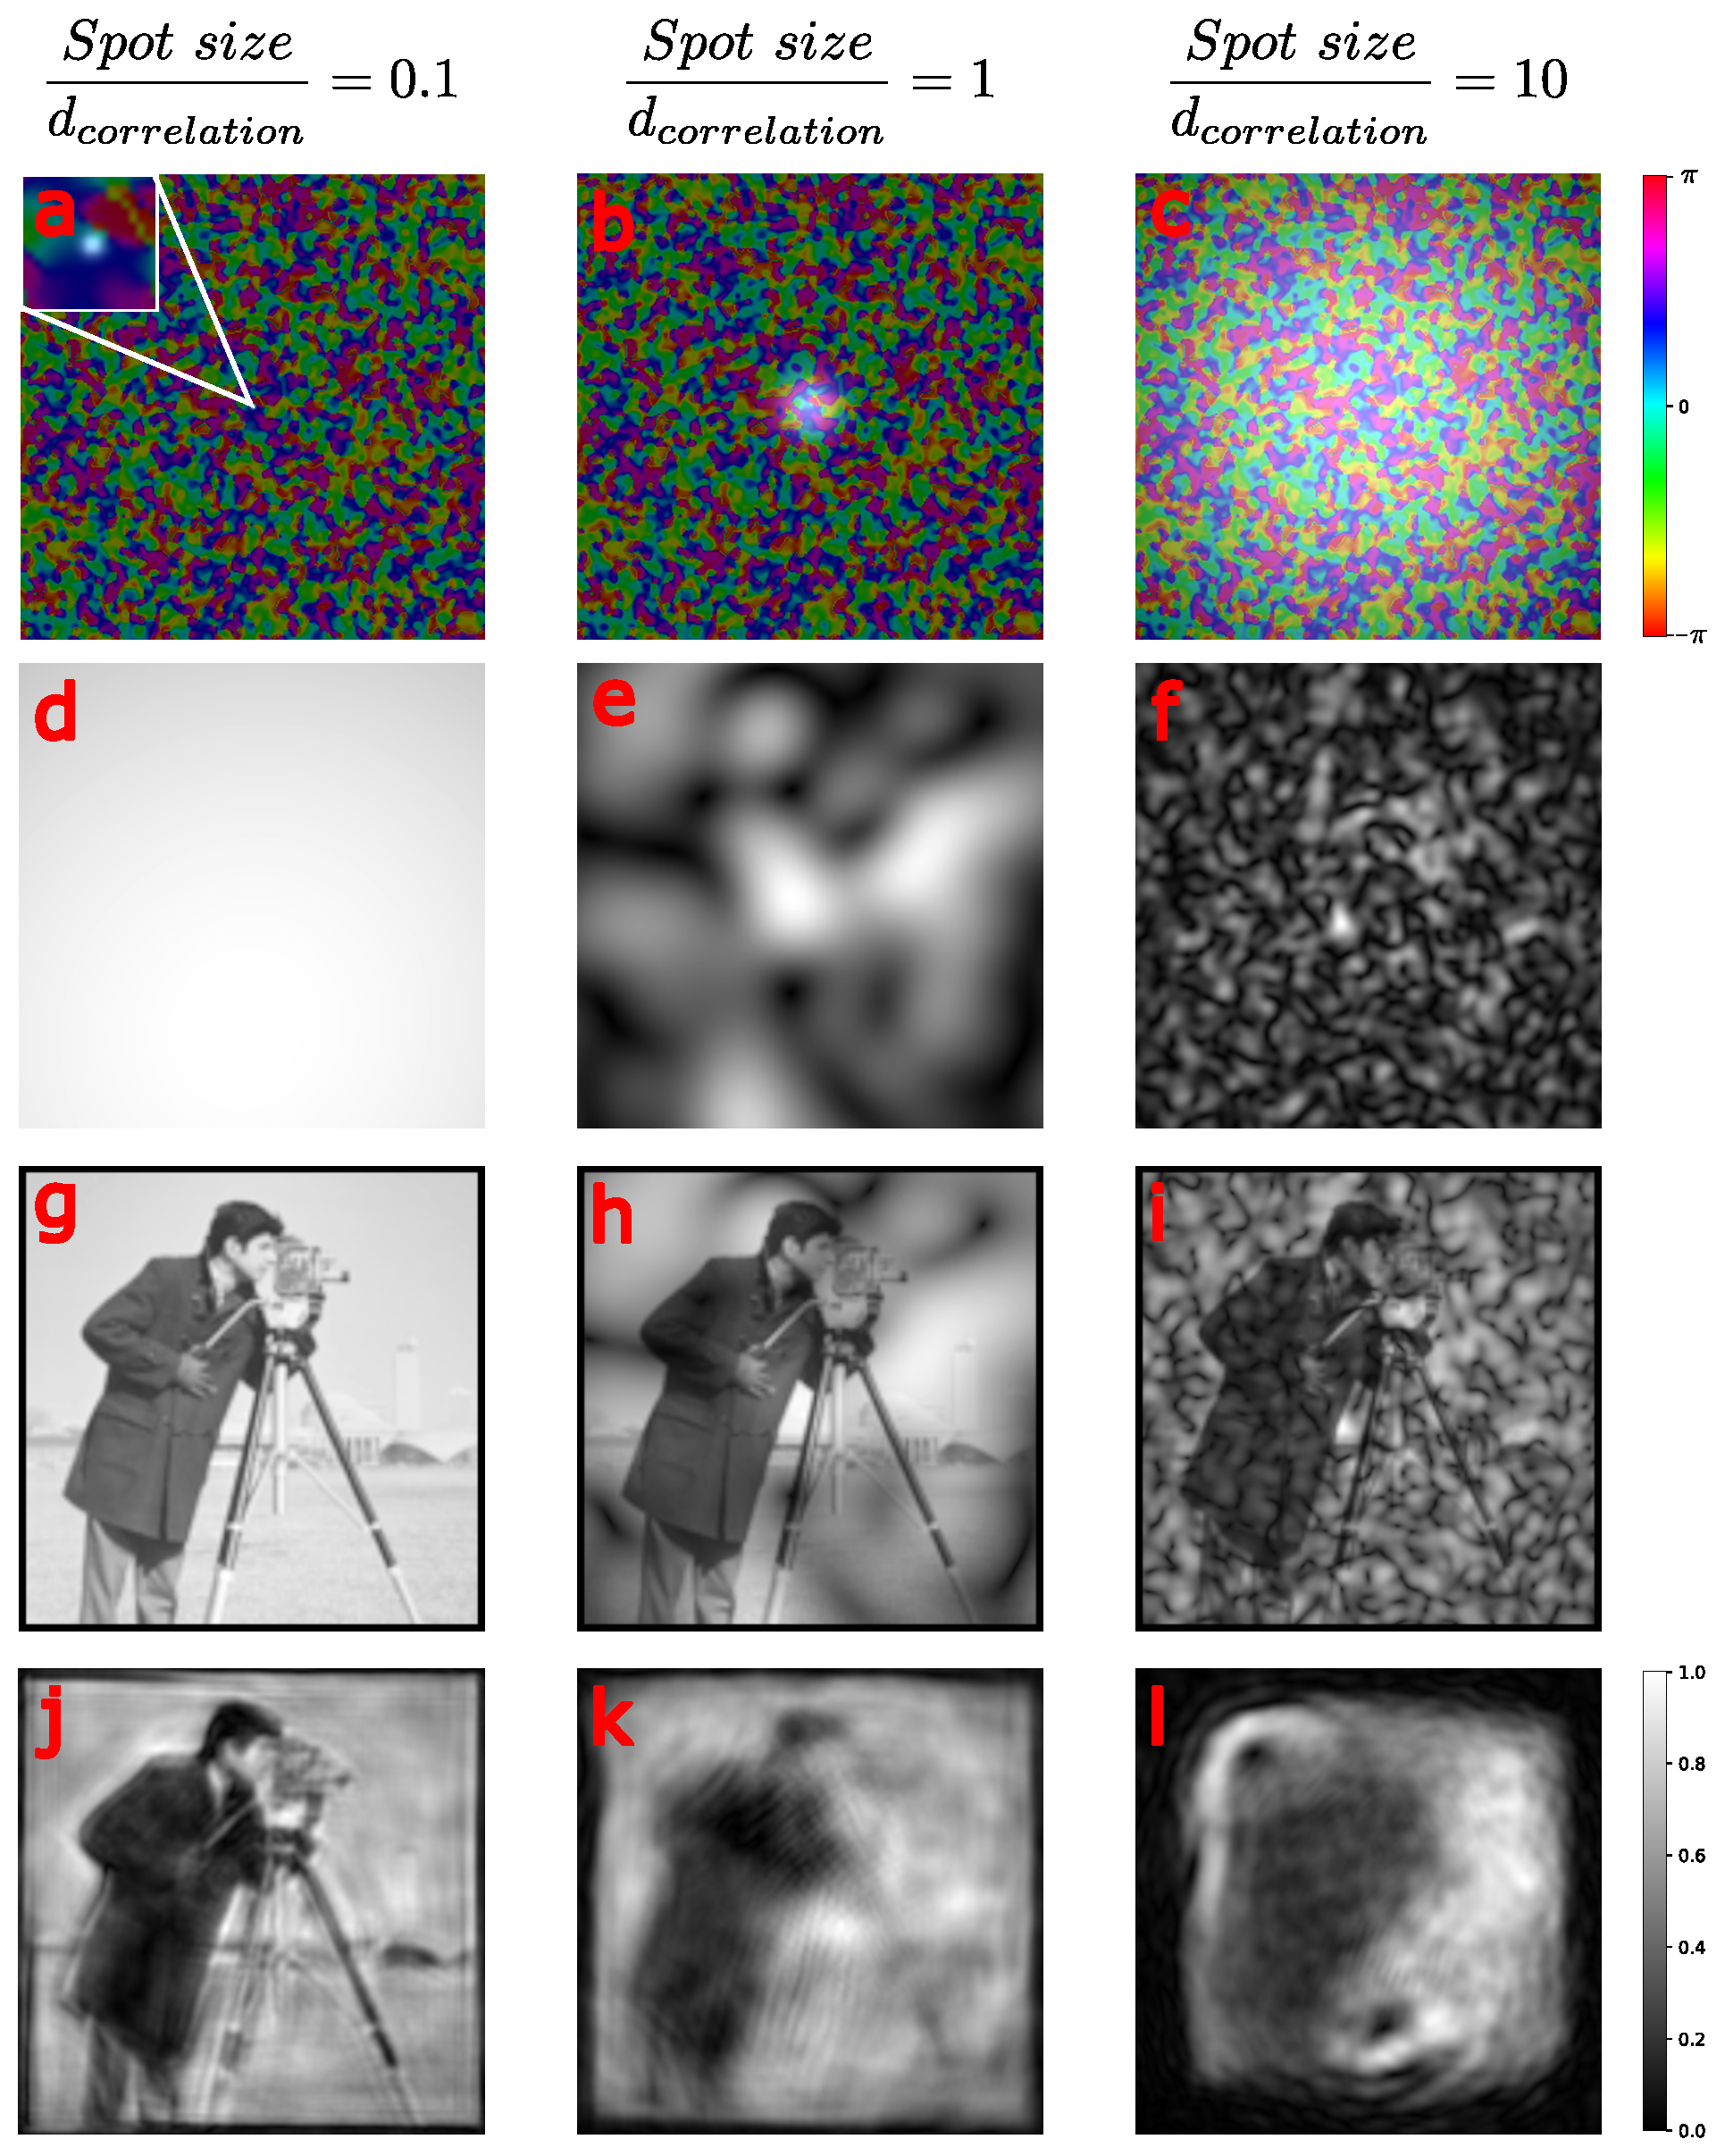
\includegraphics[width=0.99\textwidth]{supp_figures/figure_S7.pdf}
    \caption{\textbf{Effect of illumination spot size on imaging through dynamic scattering.} Numerical simulations demonstrating how the ratio of illumination spot size to diffuser correlation length affects illumination at the object plane and reconstruction quality. Each column represents a different spot size ratio: 0.1 (left), 1 (middle), and 10 (right). \textbf{a-c} Illumination phase pattern on the diffuser surface. The colorbar indicates phase values from $-\pi$ to $\pi$. The white inset in (a) shows the zoomed-in beam spot. \textbf{d-f} Resulting intensity patterns at the object plane after numerical propagation through the diffuser. The grayscale colorbar indicates normalized intensity. \textbf{g-i} Effective object (target object multiplied by the illumination pattern). \textbf{j-l} Reconstructed images after applying the I-CLASS algorithm. Note how a small spot size relative to the diffuser correlation length (left column) maintains relatively uniform illumination at the object plane, enabling high-quality reconstruction, while larger spot sizes (middle and right columns) create varying speckle patterns that degrade reconstruction quality.}
    \label{fig:spot_size}
\end{figure}

Fig.~\ref{fig:spot_size} demonstrates this principle through numerical simulation. The top row (Fig.~\ref{fig:spot_size}a-c) shows the phase pattern of the diffuser with the illumination spot superimposed for three cases: where the spot size is 0.1, 1, and 10 times the diffuser correlation length ($d_{\text{correlation}}$), respectively. The second row (Fig.~\ref{fig:spot_size}d-f) shows the resulting illumination intensity pattern at the object plane after the light has propagated through the diffuser, simulated using Fourier transform propagation.

When the illumination spot is much smaller than the diffuser correlation length (Fig.~\ref{fig:spot_size}a), it effectively samples only a single "phase patch" of the diffuser. As the diffuser rotates between realizations, this results in a relatively uniform illumination at the object plane that experiences only a global phase shift but maintains its spatial intensity pattern across different realizations. This consistency across different diffuser positions is crucial for our method to work properly. In other words, while the global phase of the illumination might change, its spatial distribution pattern remains effectively identical from one diffuser position to the next, satisfying our requirement for constant spatial illumination.

In contrast, when the illumination spot size is comparable to or larger than the diffuser correlation length (Fig.~\ref{fig:spot_size}c), the beam simultaneously samples multiple uncorrelated regions of the diffuser. This produces complex speckle patterns at the object plane that vary significantly between diffuser positions, creating a different illumination pattern for each diffuser realization. This variation violates our assumption of constant illumination in Eq. 6-7 of the main text.

The third row (Fig.~\ref{fig:spot_size}g-i) shows the effect of these illumination patterns on the effective object (the product of the object and the illumination), while the fourth row (Fig.~\ref{fig:spot_size}j-l) shows the reconstruction results. The reconstruction quality clearly degrades as the spot size increases relative to the diffuser correlation length, demonstrating the critical importance of maintaining consistent illumination across different diffuser realizations.

In our experimental implementation described in the main text, we carefully focused the beam to ensure a spot size smaller than the diffuser's correlation length ($\approx 70 \mu m$), thereby maintaining nearly constant spatial illumination patterns at the object plane across different realizations, with variations limited primarily to global phase shifts.

\newpage




\section{Dependence of Reconstruction Quality on Number of Realizations and Object Sparsity}

To study the dependence of the reconstruction quality on the number of realizations and object complexity (sparsity), we numerically simulate the reconstructions at a varying number of random realizations (M) for different object complexities (sparsity) for incoherent and coherent imaging modalities.
The results of the simulation for varying SNR values at an object sparsity are given in Figure Fig.~\ref{fig:convergence_heatmaps}

\begin{figure}[hbt!]
    \centering
    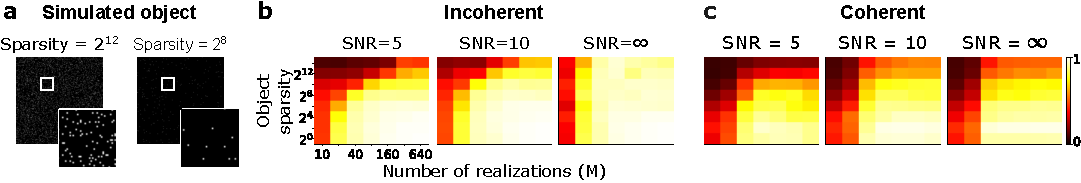
\includegraphics[width=0.98\textwidth]{supp_figures/figure_S8.pdf}
    \caption{\textbf{Reconstruction fidelity as a function of number of realizations and object sparsity.} 
    Cross-correlation scores between reconstructed and ground truth images are shown as heatmaps for different imaging scenarios. \textbf{a} Example simulated objects with different sparsity levels: $2^{12}$ (left) and $2^8$ (right) bright points. \textbf{b} Incoherent imaging results under different SNR conditions: SNR=5 (left), SNR=10 (middle), and SNR=$\infty$ (right). \textbf{c} Coherent imaging results under the same SNR conditions: SNR=5 (left), SNR=10 (middle), and SNR=$\infty$ (right). The horizontal axis shows the number of realizations (M), and the vertical axis shows object sparsity (represented as the number of bright points). Color scale indicates correlation coefficient from 0 to 1. Each data point represents the average result from 10 distinct numerical experiments with different random objects under identical parameters. For all simulations, a camera pixel count of N=350$^2$ was used.}
    \label{fig:convergence_heatmaps}
\end{figure}

These results demonstrate that sparser objects can be reconstructed with fewer realizations, while complex objects need substantially more measurements. Higher SNR conditions predictably improve reconstruction quality, and coherent imaging appears to require more measurements than incoherent imaging for equivalent fidelity.

% Our numerical simulations demonstrate a clear relationship between reconstruction quality, number of realizations (M), and object sparsity. The results show that as object complexity increases (more bright points), more realizations are needed to achieve good reconstruction quality.

%The simulations reveal several important trends:

%\begin{itemize}
 %   \item \textbf{Object Sparsity Dependence:} Sparser objects (fewer bright points) require fewer realizations for accurate reconstruction. For example, objects with only a few bright points ($2^0$ to $2^4$) can be reconstructed with high fidelity (correlation > 0.8) using just 20-40 realizations, while more complex objects ($2^{12}$ and above) require over 100 realizations to achieve similar reconstruction quality.
  %  \item \textbf{SNR Dependence:} Higher SNR enables better reconstruction with the same number of realizations. Comparing the low SNR case (panels a,d) with the noise-free case (panels c,f) shows a significant expansion of the high-correlation region (yellow) toward fewer realizations.
   % \item \textbf{Coherent vs. Incoherent Imaging:} Comparing the top row (incoherent imaging, panels a-c) with the bottom row (coherent imaging, panels d-f) reveals that coherent imaging generally requires more realizations to achieve similar reconstruction quality, particularly for objects with moderate to high complexity.
%\end{itemize}

% Based on our experimental results in the main text, where we used M=150 realizations to successfully reconstruct various objects, we can observe from these simulations that this number of realizations provides good reconstruction fidelity across a wide range of object complexities and realistic SNR conditions.



\section{Effect of Modulation Depth on Reconstruction Quality}

As discussed in Supplementary Section S2, energy conservation introduces off-diagonal correlations in the covariance matrix that can degrade reconstruction quality. We addressed this by applying variable intensity scaling across the captured frames, with multiplication factors linearly varying from 1 to 2 across frames.

To investigate the optimal range for this modulation, we conducted a study examining how different modulation depths affect reconstruction quality. For each depth value, we applied a linear scaling to our experimental data where the multiplication factor for the $m$-th frame (out of $M$ total frames) was:

\begin{equation}
    f_m = 1 + \frac{m}{M} \cdot \alpha
\end{equation}

where $\alpha$ controls the total range of modulation with corresponding modulation depth $\frac{\alpha-1}{\alpha+1}$.

\begin{figure}[htb!]
	\centering
	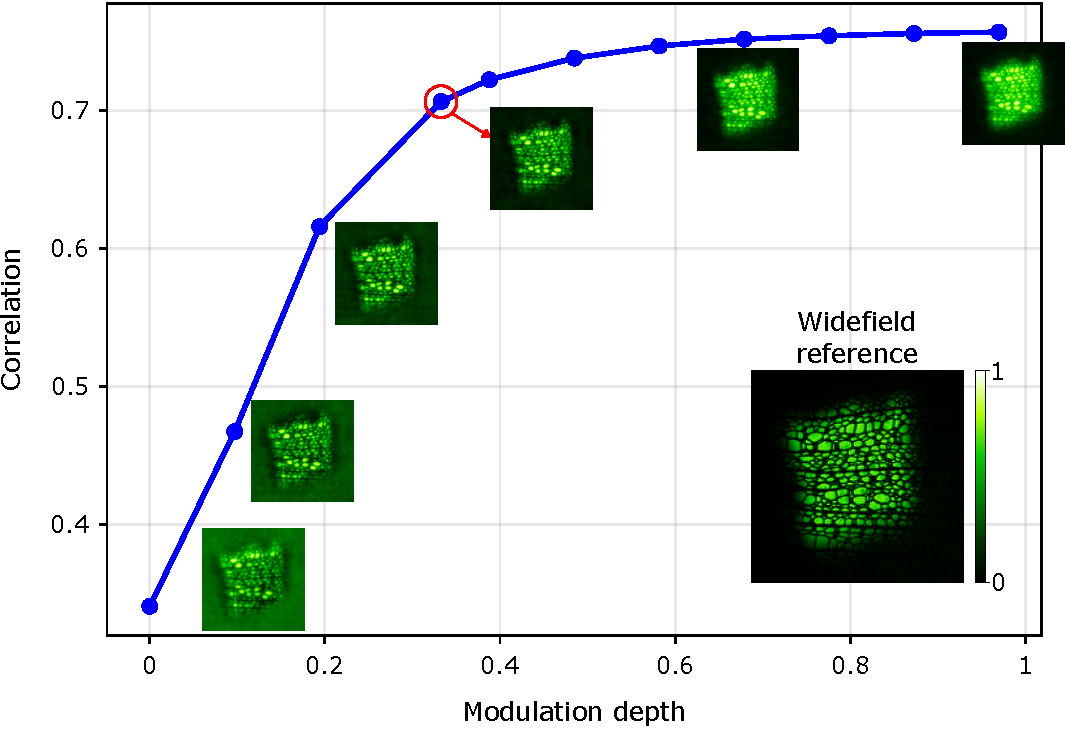
\includegraphics[width=0.85\textwidth]{supp_figures/Figure_S9.pdf}
    \caption{\textbf{Effect of modulation depth on reconstruction quality.} The similarity score shows how reconstruction quality improves with increasing modulation depth. Example reconstructions demonstrate the progressive elimination of background haze as modulation increases, while at higher modulation depths, some haze begins to appear within the object itself. The red circle indicates our chosen modulation depth, which offers a good trade-off in this balance.}
\end{figure}

Our results show that without modulation (depth = 0), reconstructions exhibit significant background haze. As modulation increases, this background haze diminishes progressively. However, at higher modulation depths, while the background continues to improve, some haze begins to appear within the object itself.

The multiplication factor range of 1 to 2 used in our main experiments provides an effective trade-off between these competing effects. However, depending on specific application requirements, users might prefer different modulation depths to prioritize either background cleanliness or internal object clarity.

\section*{Captions for movies}

\subsection*{Video S1.}
Measured experimental uncorrected frames of the target object, as presented in Fig.~2b-e of the main text, displayed alongside their estimated PSFs and the I-CLASS reconstruction.

\subsection*{Video S2.}
Measured experimental uncorrected frames of the target object, as presented in Fig.~2f-i of the main text, displayed alongside their estimated PSFs and the I-CLASS reconstruction.

\newpage


\bibliography{bib}

\end{document}
